\chapter{Penulisan dalam LaTex}

Dalam bab ini dituliskan tata cara penulisan jurnal dalam format latex. Latex merupakan salah satu alat untuk membantu proses pembuatan jurnal ilmiah yang cepat dan sesuai dengan format. Dengan latex kita bisa melakukan penghematan waktu penulisan karena tidak perlu terjebak dalam kesibukan formating jurnal. Mungkin pada pertama kali kita akan terasa kesulitan karena baru belajar menggunakan scripting latex. Tapi setelah terbiasa. Kita akan mulai ketagihan menggunakannya.


\section{Standar Format Latex}
Format latex yang dipakai pada buku ini adalah format khusus yang sudah dibagi dengan folder standar dan file standar agar mempermudah dalam pengerjaan. Beberapa Aturan yang ada di dalam format ini antara lain :
\begin{enumerate}

    \item file disimpan dalam format ber ekstensi .tex per chapter masing2 di folder section

    \item gambar disimpan dalam folder figures dengan namagambar

	\item referensi BibTex disimpan di file bernama references.bib
	
\end{enumerate}

\section{Pengaturan Bab dan Sub Bab}

Penyebutan subbab dan subsubbab diatur dengan cara : \\
    judul sub bab : \\ 
    \verb|\section{nama sub bab}| \\
    judul sub sub bab ditulis dengan :\\ 
    \verb|\subsection{judul sub sub bab} | \\
    judul sub sub sub bab ditulis dengan : \\ \verb|\subsubsection{Judul sub sub sub bab} | \\
    contoh :
    \begin{verbatim}
    \section{Sejarah Peta}
Perkembangan peta dunia tidak luput dari para ahli 
geografi dan kartografi. Peta dunia yang populer pada saat 
ini merupakan 
kontribusi dari para 
pembuat peta sebelumnya

\subsection{Ptolemy's}
Ptolemy's diduga membuat peta pada abad ke 2
\end{verbatim}


\section{Melakukan Sitasi}

Cara yang paling cepat dan mudah untuk membuat daftar pustaka adalah dengan menggunakan Google Schoolar. Referensi yang sudah kita baca, kita masukkan ke judulnya ke pencarian dari google scholar,scholar.google.com. Kemudian, setiap referensi yang diambil, maka tambahkan dan tuliskan ke dalam file bernama references.bib yang berisi kumpulan bibTex dari referensi. Gunakan standar pengutipan yang baik dan benar,dan hindari plagiasi. Cara menggunakan dan mengambil bibtex sudah dijelaskan pada BAB I. 

Referensi disebutkan dengan menyebutkan nama di dalam bibtex setelah tanda kurung kurawal buka dan sebelum tanda koma. Contoh, Jika Bibtex sudah diinputkan kedalam reference.bib seperti ini :
\begin{verbatim}
@inproceedings{ganapathi2006windows,
  title={Windows XP Kernel Crash Analysis.},
  author={Ganapathi, Archana and Ganapathi, 
  Viji and Patterson, David A},
  booktitle={LISA},
  volume={6},
  pages={49--159},
  year={2006}
}
\end{verbatim}
Maka penulisan kalimat di jurnal : \\
Dalam sebuah artikel dari Ganapathi yang 
menyebutkan bahwa komputasi adalah keniscayan \verb|\cite{ganapathi2006windows}|.


\section{Memasukkan Gambar}

Pastikan gambar sudah diberi label seperti skrip di bawah ini dengan tag label \verb|\label{labelgambar}| . Gambar disebutkan di dalam artikel dengan format sesuai labelnya yaitu \verb|\ref{labelgambar}|. Gambar diselipkan dengan menambahkan blok sintaks :
    \begin{verbatim}
    \begin{figure}[ht]
    \centerline{\includegraphics[width=1\textwidth]
    {figures/namagambar.JPG}}
    \caption{penjelasan keterangan gambar.}
    \label{labelgambar}
    \end{figure}
    
   	Contoh dalam narasi di dalam paragraf yaitu :
    Pada gambar \ref{labelgambar} dijelaskan bahwa 
    sistem operasi memiliki 3 versi.
    \end{verbatim}

Dan jangan lupa, dilarang keras menggunakan kalimat penyebutan relatif terhadap gambar. Contoh : gambar di bawah ini. Tapi gunakan kalimat penyebutan referensi nomor gambarnya. Contoh : Bisa dilihat di Gambar 1.

\section{Urutan Nomor dan Poin}

Penggunaan nomor urut atau yang sering kita dengar dengan istilah numbering. Serta penggunaan poin atau yang sering disebut sebagai bullet adalah sebagai berikut. Untuk nomor gunakan tag enumerate. Sedangkan untuk bullet atau poin menggunakan tag itemize. Sebagai contoh :
\begin{verbatim}
berikut nama anggota kelompok
\begin{enumerate}
\item darso
\item karyo
\item doyok
\end{enumerate}

\begin{enumerate}
\item
This is the first item in the numbered list.

\item
This is the second item in the numbered list.
\end{enumerate}

\begin{itemize}
\item
This is the first item in the itemized list.

\item
This is the first item in the itemized list.
This is the first item in the itemized list.
This is the first item in the itemized list.
\end{itemize}

\begin{itemize}
\item[]
This is the first item in the itemized list.

\item[]
This is the first item in the itemized list.
This is the first item in the itemized list.
This is the first item in the itemized list.
\end{itemize}
\end{verbatim}
    
\section{Karakter Khusus}

spesial karakter menggunakan tanda `\verb|\|' didepannya contoh :
\begin{verbatim}
\& 
\% 
\$ 
\#  
\{ \}
\_
\end{verbatim}

Tanda pentik menggunakan petik pembuka dengan menggunakan petik diatas angka 1. 
Dan petik penutup dengan menggunakan tanda petik satu biasa.
\begin{verbatim}
\"dalam petik\"
`dalam petik'
\end{verbatim} 
Apostrop atau tanda petik satu pada penggunaan kata bahasa inggris sering digunakan. Tanpa petik satu sudah bisa terbaca dan dipakai sehingga tidak perlu ada karakter khusus. Apabila ada error pastikan anda mengetik tanpa petik satu yang benar bukan hasil copas dari file lain. Sehingga apabila diimplementasikan menjadi :
\begin{verbatim}
`It's a nice day!'
\end{verbatim} 
Hasilnya akan menjadi : `It's a nice day!'

Jika spesial karakter menjadi banyak atau satu baris gunakan verb
contoh :
\begin{verbatim}
\verb|%$'%&$&'%'%'%&'%|
\end{verbatim}

\section{Penggunaan Tabel}

untuk tabel gunakan table , dan jangan lupa tabel di referensikan pada kalimat berdasarkan labelnya. 
contoh:
\begin{verbatim}
ini merupakan contoh tabel \ref{table:contoh} ukuran kecil.
\begin{table}[h]
\caption{Small Table}
\centering
\begin{tabular}{ccc}
\hline
one&two&three\\
\hline
C&D&E\\
\hline
\end{tabular}
\label{table:contoh}
\end{table}
    \end{verbatim}

\section{Penggunaan Rumus}

untuk rumus gunakan tag equation dan di referensikan pada kalimat dengan tag ref sesuai labelnya. contoh:
\begin{verbatim}
Luas permukaan dijelaskan pada rumus \ref{eq:1}.Volume dijelaskan 
pada rumus \ref{eq:2}.
$L$ merupakan luas, $\pi$ adalah 3,14.
\begin{equation}\label{eq:1}
     L = 4 \pi r^2 \,
\end{equation}
 \begin{equation}\label{eq:2}
     V = \frac{4}{3}\pi r^3
\end{equation}
\end{verbatim}
Hasil dari skrip diatas menjadi :

Luas permukaan dijelaskan pada rumus \ref{eq:1}.Volume dijelaskan 
pada rumus \ref{eq:2}.
$L$ merupakan luas, $\pi$ adalah 3,14.
\begin{equation}\label{eq:1}
     L = 4 \pi r^2 \,
\end{equation}
 \begin{equation}\label{eq:2}
     V = \frac{4}{3}\pi r^3
\end{equation}
 
Contoh selanjutnya adalah, apabila terdapat simbol-simbol matematika maka kita bisa melihat contoh rumus berikut :

    \begin{verbatim}
		Rumus \ref{eq:3} adalah contoh penggunaan rumus mean atau rata-rata .
		Sedangkan rumus \ref{eq:4} adalah Median untuk ganjil  
		dan untuk genap di rumus \ref{eq:5}.
		Dan modus \ref{eq:6}
		\begin{equation}\label{eq:3}
		 \Bar{x} = \frac{X_1+X_2+X_3+...+X_n}{n}    
		\end{equation}
		\begin{equation}\label{eq:4}
		    \Bar{x} = \frac{n+1}{2}
		\end{equation}
		\begin{equation}\label{eq:5}
		    \Bar{x} = \frac{1}{2} [\frac{n}{2}+\langle\frac{n}{2}+1\rangle]
		\end{equation}
		\begin{equation}\label{eq:6}
		    L + i [\frac{d_1}{d_1d_2}]
		\end{equation}
    \end{verbatim}

Hasil dari script diatas adalah :

Rumus \ref{eq:3} adalah contoh penggunaan rumus mean atau rata-rata .
Sedangkan rumus \ref{eq:4} adalah Median untuk ganjil  
dan untuk genap di rumus \ref{eq:5}.
Dan modus \ref{eq:6}
\begin{equation}\label{eq:3}
 \Bar{x} = \frac{X_1+X_2+X_3+...+X_n}{n}    
\end{equation}
\begin{equation}\label{eq:4}
    \Bar{x} = \frac{n+1}{2}
\end{equation}
\begin{equation}\label{eq:5}
    \Bar{x} = \frac{1}{2} [\frac{n}{2}+\langle\frac{n}{2}+1\rangle]
\end{equation}
\begin{equation}\label{eq:6}
    L + i [\frac{d_1}{d_1d_2}]
\end{equation}

Daftar lengkap simbol matematis bisa dilihat di lampiran buku ini.



\section{Kode Program}
untuk kode program menggunakan verbatim
\begin{verbatim}
\ begin{verbatim}
a = "anu"
b = "itu"
c = a + b
print(c) 
\ end{verbatim}
\end{verbatim}


\section{Pengaturan Ukuran Kertas dan Margin}
Apabila margin tidak sesuai atau ukuran kertas tidak sesuai latex memiliki settingan bawaan. Biasanya kebanyakan para pembuat template memakai package saja. Tapi masih ada juga yang mendefinisikan ukuran kertas dan margin tanpa menggunakan package. Gambar \ref{marginsize} menunjukkan bagaimana perintah untuk penyesuaian margin dan ukuran kertas.

  	\begin{figure}[ht]
  \centerline{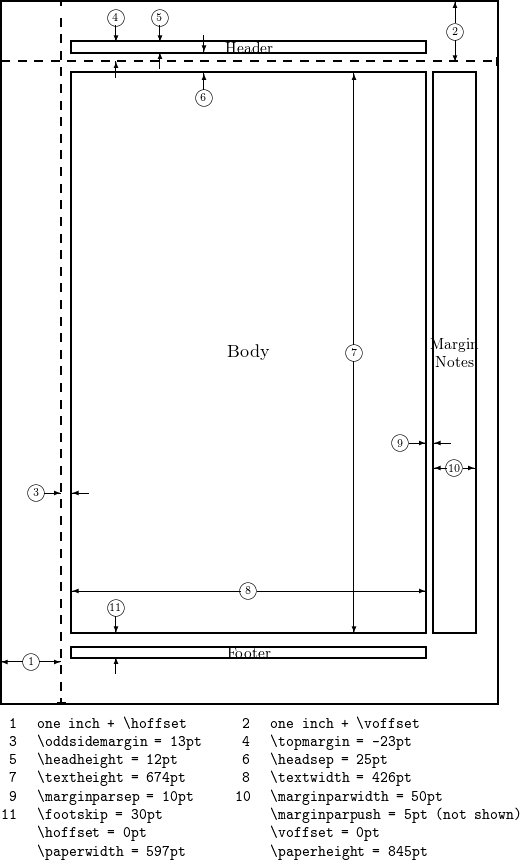
\includegraphics[width=.5\textwidth]
  {figures/custommarginlatex.png}}
  \caption{Perintah pengaturan margin dan ukuran kertas.}
  \label{marginsize}
  \end{figure}


